% Copyright 2021  Ed Bueler

\documentclass[xcolor={svgnames},
               hyperref={colorlinks,citecolor=DeepPink4,linkcolor=FireBrick,urlcolor=Maroon}]
               {beamer}

\mode<presentation>{
  \usetheme{Madrid}
  \usecolortheme{seagull}
  \setbeamercovered{transparent}
  \setbeamerfont{frametitle}{size=\large}
}

\setbeamercolor*{block title}{bg=red!10}
\setbeamercolor*{block body}{bg=red!5}

\usepackage[english]{babel}
\usepackage[latin1]{inputenc}
\usepackage{times}
\usepackage[T1]{fontenc}
% Or whatever. Note that the encoding and the font should match. If T1
% does not look nice, try deleting the line with the fontenc.

\usepackage{empheq}
\usepackage{xspace}
\usepackage{verbatim,fancyvrb}

\usepackage{tikz}
\usetikzlibrary{shapes,arrows.meta,decorations.markings,decorations.pathreplacing,fadings,positioning}


% If you wish to uncover everything in a step-wise fashion, uncomment
% the following command:
%\beamerdefaultoverlayspecification{<+->}

\newcommand{\ba}{\mathbf{a}}
\newcommand{\bb}{\mathbf{b}}
\newcommand{\bc}{\mathbf{c}}
\newcommand{\bbf}{\mathbf{f}}
\newcommand{\bg}{\mathbf{g}}
\newcommand{\bn}{\mathbf{n}}
\newcommand{\bq}{\mathbf{q}}
\newcommand{\br}{\mathbf{r}}
\newcommand{\bx}{\mathbf{x}}
\newcommand{\by}{\mathbf{y}}
\newcommand{\bv}{\mathbf{v}}
\newcommand{\bu}{\mathbf{u}}
\newcommand{\bw}{\mathbf{w}}

\newcommand{\bF}{\mathbf{F}}
\newcommand{\bG}{\mathbf{G}}
\newcommand{\bQ}{\mathbf{Q}}

\newcommand{\grad}{\nabla}
\newcommand{\Div}{\nabla\cdot}
\newcommand{\minmod}{\operatorname{minmod}}

\newcommand{\CC}{\mathbb{C}}
\newcommand{\RR}{\mathbb{R}}

\newcommand{\ddt}[1]{\ensuremath{\frac{\partial #1}{\partial t}}}
\newcommand{\ddx}[1]{\ensuremath{\frac{\partial #1}{\partial x}}}
\newcommand{\Matlab}{\textsc{Matlab}\xspace}
\newcommand{\Octave}{\textsc{Octave}\xspace}
\newcommand{\eps}{\epsilon}

\newcommand{\ip}[2]{\left<#1,#2\right>}

\newcommand{\xiphalf}{{x_{i+\frac{1}{2}}}}
\newcommand{\ximhalf}{{x_{i-\frac{1}{2}}}}
\newcommand{\Fiphalf}{{F_{i+\frac{1}{2}}}}
\newcommand{\Fimhalf}{{F_{i-\frac{1}{2}}}}
\newcommand{\Fiphalfn}{{F^n_{i+\frac{1}{2}}}}
\newcommand{\Fimhalfn}{{F^n_{i-\frac{1}{2}}}}

\newcommand{\trefcolumn}[1]{\begin{bmatrix} \phantom{x} \\ #1 \\ \phantom{x} \end{bmatrix}}
\newcommand{\trefmatrixtwo}[2]{\left[\begin{array}{c|c|c} & & \\ #1 & \dots & #2 \\ & & \end{array}\right]}
\newcommand{\trefmatrixthree}[3]{\left[\begin{array}{c|c|c|c} & & & \\ #1 & #2 & \dots & #3 \\ & & & \end{array}\right]}
\newcommand{\trefmatrixgroups}[4]{\left[\begin{array}{c|c|c|c|c|c} & & & & & \\ #1 & \dots & #2 & #3 & \dots & #4 \\ & & & & & \end{array}\right]}

\newcommand{\blocktwo}[4]{\left[\begin{array}{c|c} #1 & #2 \\ \hline #3 & #4 \end{array}\right]}

\newcommand{\bqed}{{\color{blue}\qed}}
\newcommand{\ds}{\displaystyle}

\newcommand\mynum[1]{{\renewcommand{\insertenumlabel}{#1}%
      \usebeamertemplate{enumerate item} \,}}


\title{Getting started with machine learning}

\subtitle{({one little artificial neural net})}

\author{Ed Bueler}

\institute[UAF]{MATH 692 Mathematics for Machine Learning \\ UAF}

\date[Spring 2022]{13 January 2022}

%\titlegraphic{\begin{picture}(0,0)
%    \put(0,180){\makebox(0,0)[rt]{\includegraphics[width=4cm]{figs/software.png}}}
%  \end{picture}
%}

%% this nonsense needed to start section counter at 0; see
%% https://tex.stackexchange.com/questions/170222/change-the-numbering-in-beamers-table-of-content
\makeatletter
\patchcmd{\beamer@sectionintoc}
  {\ifnum\beamer@tempcount>0}
  {\ifnum\beamer@tempcount>-1}
  {}
  {}
%\beamer@tocsectionnumber=-1
\makeatother


\begin{document}
\beamertemplatenavigationsymbolsempty

\begin{frame}
  \maketitle
\end{frame}

\begin{frame}{today's talk}

\begin{itemize}
\item \alert{my topic:} {\small how this $\downarrow$ neural network does this $\downarrow$ classification task}

\medskip
\hspace{5mm} 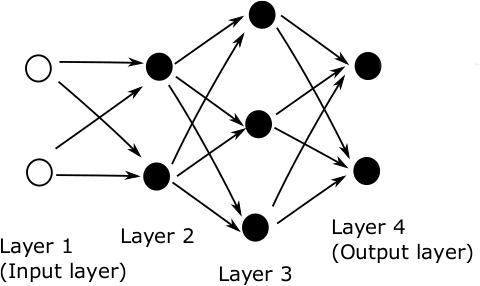
\includegraphics[height=25mm]{figs/network.png} \hfill 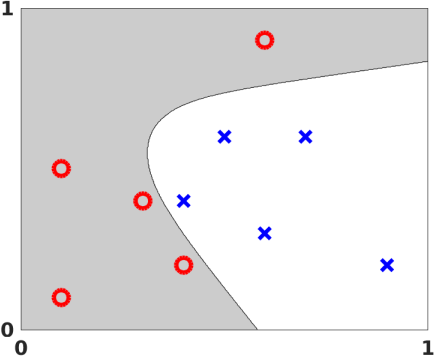
\includegraphics[height=23mm]{figs/classification} \hspace{10mm}

\medskip
\item an \alert{example} from this $\downarrow$ paper:

\medskip

HH19 \, $=$ \, 
\begin{minipage}[t]{0.75\textwidth} \footnotesize
C.~F.~Higham \& D.~J.~Higham (2019). \href{http://www.math.stonybrook.edu/~bishop/classes/math533.S21/MachineLearning/SIAMreview.pdf}{\emph{Deep learning: An introduction for applied mathematicians.}} SIAM Review, 61(4), 860-891
\end{minipage}
\end{itemize}
\end{frame}


\begin{frame}{today's talk}

\begin{itemize}
\item \alert{goal for today:} know the meanings of

\medskip
\small
\qquad \begin{tabular}{ll}
\emph{artificial neuron} \qquad & \emph{activation function} \\
\emph{weight matrix} & \emph{bias vector} \\
\emph{back-propagation} & \emph{stochastic gradient method}
\end{tabular}

\medskip
\item which standard mathematical concept(s) match these buzzwords?
\end{itemize}
\end{frame}


\begin{frame}{big caveat}

\begin{itemize}
\item I am no expert on what I am talking about here
\item many in room know more than me
\item I volunteered to give one intro talk, that's all!
\end{itemize}
\end{frame}


\begin{frame}{\emph{participant}-driven seminar logistics}

\begin{itemize}
\item sign-up sheet!
\item my existing webpages:
    \begin{itemize}
    \item[$\circ$] \href{http://bueler.github.io/M692S22/index.html}{\texttt{bueler.github.io/M692S22}}
    \item[$\circ$] \href{https://github.com/bueler/ml-seminar}{\texttt{github.com/bueler/ml-seminar}}
    \end{itemize}
\item in-person or hybrid?
    \begin{itemize}
    \item[$\circ$] is this classroom adequate?
    \end{itemize}
\item what will be the topics?
    \begin{itemize}
    \item[$\circ$] are there out-of-bounds topics?
    \item[$\circ$] who is volunteering to talk?
    \end{itemize}
\end{itemize}
\end{frame}


\begin{frame}{Outline}
  \tableofcontents[hideallsubsections]
\end{frame}

\section{a single artificial neuron}

\begin{frame}{one artificial neuron $=$ nonlinear-ized inner product}

\begin{columns}
\begin{column}{0.55\textwidth}
\begin{itemize}
\item given (column) vectors $v,w \in \RR^n$
\item recall \emph{inner product}:
    $$\ip{{\color{blue} w}}{v} = {\color{blue} w}^\top v = \sum_{j=1}^n {\color{blue} w_j} v_j$$
\item apply a nonlinear function $\sigma: \RR^1 \to \RR^1$:
\only<1>{
\begin{equation*}
{\color{red} a} = \sigma\left(\sum_{j=1}^n {\color{blue} w_j} v_j\right) \in \RR^1
\end{equation*}
}
\only<2>{
\begin{equation*}
{\color{red} a} = \sigma\left(\sum_{j=1}^n {\color{blue} w_j} v_j + {\color{ForestGreen} b}\right) \in \RR^1
\end{equation*}
}
    \begin{itemize}
    \item<2>[$\circ$] detail: add a bias ${\color{ForestGreen} b} \in \RR^1$
    \item<2>[$\circ$] that's it! an \alert{artificial neuron}
    \end{itemize}
\end{itemize}
\end{column}
\begin{column}{0.45\textwidth}
\only<1>{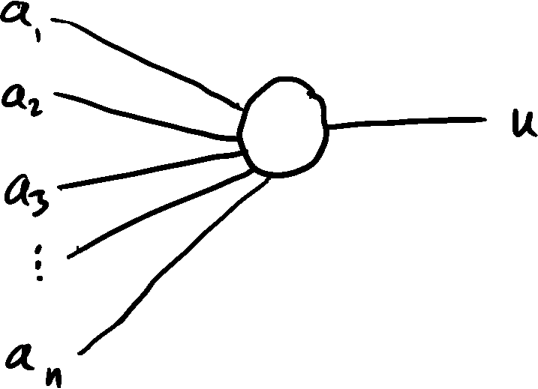
\includegraphics[width=\textwidth]{figs/single-neuron}}
\only<2>{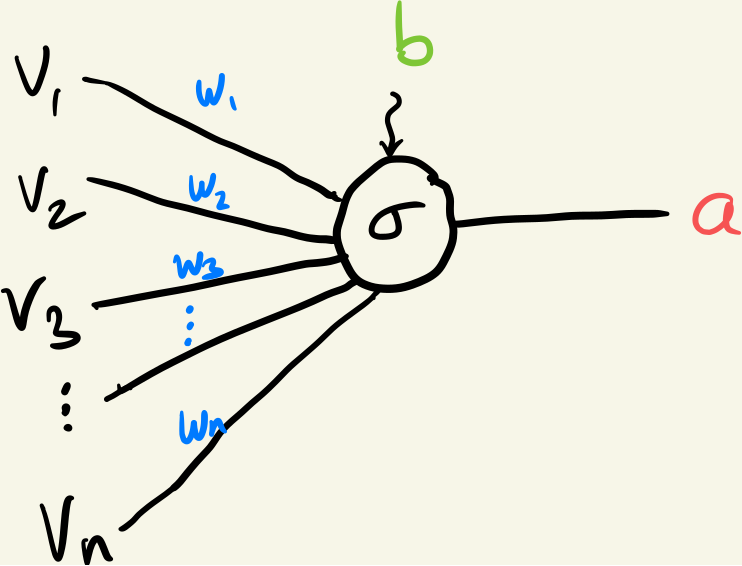
\includegraphics[width=\textwidth]{figs/b-single-neuron}}
\end{column}
\end{columns}
\end{frame}


\begin{frame}{neuron roles}

\begin{columns}
\begin{column}{0.55\textwidth}
\begin{itemize}
\item $v$ is input
\item \alert{weights} ${\color{blue} w}$ and \alert{biases} ${\color{ForestGreen} b}$ are parameters
    \begin{itemize}
    \item[$\circ$] they need \alert{training}
    \end{itemize}
\item the \alert{activation function} $\sigma$ is fixed
\item the output ${\color{red} a}$ is the \alert{activation} of the neuron
\end{itemize}
\end{column}
\begin{column}{0.45\textwidth}
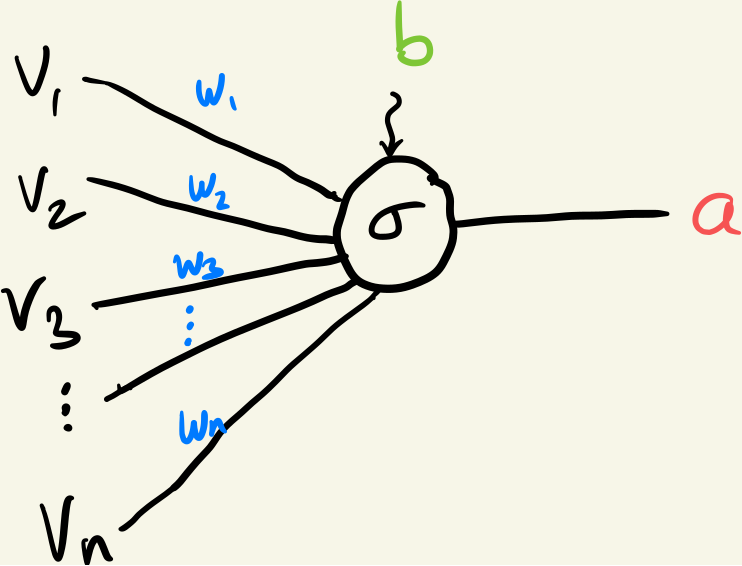
\includegraphics[width=\textwidth]{figs/b-single-neuron}
\end{column}
\end{columns}
\end{frame}


\begin{frame}{nonlinear activation function}

\begin{center}
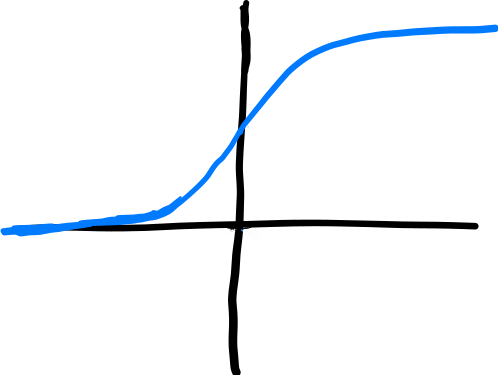
\includegraphics[height=30mm]{figs/sigmoid} \hspace{10mm} 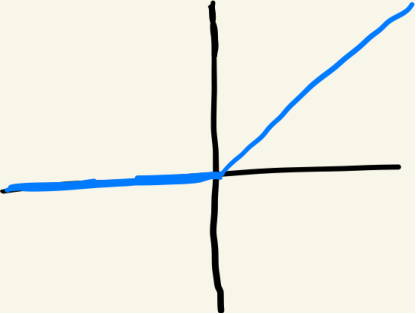
\includegraphics[height=30mm]{figs/relu}
\end{center}

\begin{itemize}
\item $\sigma$ is the \alert{activation function}
\item possibilities:
    \begin{itemize}
    \item[$\circ$] \alert{sigmoid}, e.g.\qquad $\displaystyle \sigma(z) = \frac{1}{1 + e^{-z}}$ \quad (left)
    \item[$\circ$] \alert{rectified linear unit (ReLU)},\qquad $\displaystyle \sigma(z) = \begin{cases} z, & z > 0 \\ 0, & z \le 0 \end{cases}$ \quad (right)
    \end{itemize}
\item $\sigma$ is increasing, with bounded derivative
\end{itemize}
\end{frame}


\begin{frame}{a trained neuron}

\begin{columns}
\begin{column}{0.55\textwidth}
\begin{itemize}
\item a \alert{trained neuron} is one with known parameters $w,b$
\item so $a:\RR^n \to \RR^1$ is a known function:
    $${\color{red} a} = \sigma(v)$$

    \begin{itemize}
    \item[$\circ$] similar cost to inner product
    \item[$\circ$] backward stable
    \end{itemize}
\item one might write
    $${\color{red} a} = \sigma(v;{\color{blue} w},{\color{ForestGreen} b})$$
to make dependence on parameters clear
\end{itemize}
\end{column}
\begin{column}{0.45\textwidth}
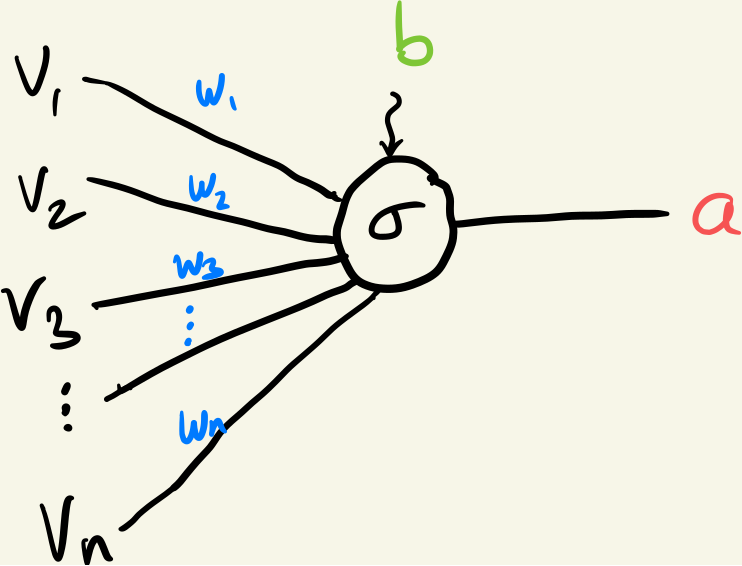
\includegraphics[width=\textwidth]{figs/b-single-neuron}
\end{column}
\end{columns}
\end{frame}


\section{forward through a neural net}

\begin{frame}{Outline}
  \tableofcontents[hideallsubsections,currentsection]
\end{frame}


\begin{frame}{feed-forward networks}

\begin{center}
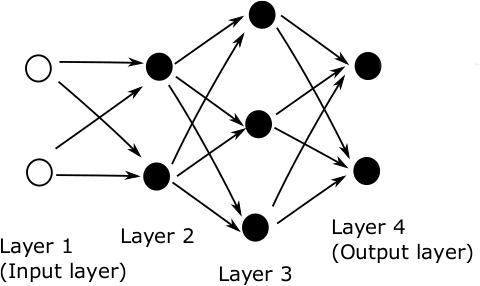
\includegraphics[height=30mm]{figs/network}
\end{center}

\begin{itemize}
\item assumption made here: considering only \alert{feed-forward} networks
    \begin{itemize}
    \item[$\circ$] edges only connect consecutive layers, in order
    \item[$\circ$] in language of graph theory: connected, directed acyclic graph (DAG) which is equal to its own transitive reduction \dots I think
    \item[$\circ$] \alert{feed-forward} versus \alert{recurrent}
    \end{itemize}
\end{itemize}
\end{frame}


\begin{frame}{network notation}

\begin{center}
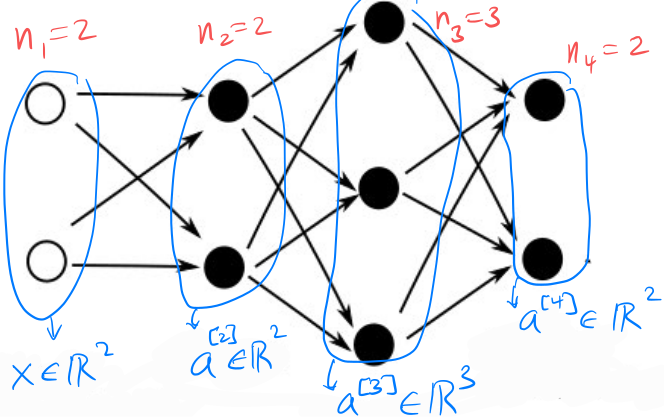
\includegraphics[height=35mm]{figs/state-notation}
\end{center}

\begin{itemize}
\item notation from HH19
\item ${\color{red} n_\ell}$ is number of neurons in layer $\ell=1,\dots,L$
    \begin{itemize}
    \item[$\circ$] $\ell=1$ is \alert{input} layer
    \item[$\circ$] input values equal first-layer activations: $x = {\color{blue} a^{[1]}} \in \RR^{{\color{red} n_1}}$)
    \item[$\circ$] $\ell=L$ is \alert{output} layer
    \item[$\circ$] output values equal $L$th-layer activations: $y = {\color{blue} a^{[L]}} \in \RR^{{\color{red} n_L}}$)
    \end{itemize}
\item activations in layer $\ell$ form a vector ${\color{blue} a^{[\ell]}} \in \RR^{{\color{red} n_\ell}}$
    \begin{itemize}
    \item[$\circ$] ${\color{blue} a_j^{[\ell]}}$ is activation of neuron $j$ in layer $\ell$
    \item[$\circ$] we label a neuron by its activation: ``neuron ${\color{blue} a_j^{[\ell]}}$''
    \end{itemize}
\end{itemize}
\end{frame}


\begin{frame}{weight notation}

\begin{center}
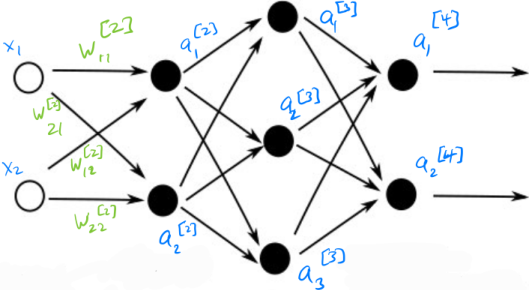
\includegraphics[height=40mm]{figs/weight-notation}
\end{center}

\begin{itemize}
\item weight ${ \color{ForestGreen} w_{jk}^{[\ell]} }$ on the edge from neuron ${\color{blue} a_k^{[\ell-1]}}$ to neuron ${\color{blue} a_j^{[\ell]}}$
\item thus
    $${\color{blue} a_j^{[\ell]}} = \sigma\left(\sum_{k=1}^{n_{\ell-1}} {\color{ForestGreen} w_{jk}^{[\ell]}} {\color{blue} a_k^{[\ell-1]}} + b_j\right)$$
\item which suggests matrix-vector multiplication!
\end{itemize}
\end{frame}


\begin{frame}{weight notation using vectors and matrices}

\begin{center}
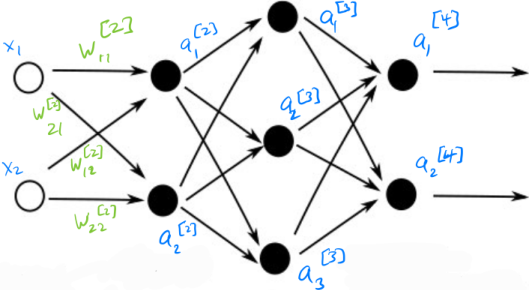
\includegraphics[height=35mm]{figs/weight-notation}
\end{center}

\begin{itemize}
\item one row vector ${\color{ForestGreen} w^\top}$ of weights for each neuron
\item neurons in a layer deserve a matrix:
    $${\color{ForestGreen} W^{[\ell]}} = \left(\text{weights into layer $\ell$}\right) = \begin{bmatrix} {\color{ForestGreen} w_{jk}^{[\ell]}} \end{bmatrix}$$

    \begin{itemize}
    \item[$\circ$] ${\color{ForestGreen} W^{[\ell]}}$ is $n_{\ell}\times n_{\ell-1}$
    \end{itemize}
\item assume $\sigma$ applied entrywise, thus with biases $b^{[\ell]} \in \RR^{n_{\ell}}$,
    $${\color{blue} a^{[\ell]}} = \sigma\left({\color{ForestGreen} W^{[\ell]}} {\color{blue} a^{[\ell-1]}} + b^{[\ell]}\right)$$
\end{itemize}
\end{frame}


\begin{frame}{forward pass = nonlinear-ized matrix multiplication}

\begin{center}
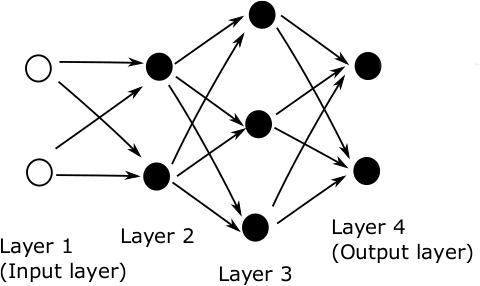
\includegraphics[height=25mm]{figs/network}
\end{center}

\begin{itemize}
\item for this small $L=4$ network:
\begin{align*}
y = a^{[4]} &= \sigma\left(W^{[4]} a^{[3]} + b^{[4]}\right) = \dots \\
            &= \sigma\left(W^{[4]} \sigma\left(W^{[3]} \sigma\left(W^{[2]} a^{[1]} + b^{[2]}\right) + b^{[3]}\right) + b^{[4]}\right) \\
            &= \sigma\left(W^{[4]} \sigma\left(W^{[3]} \sigma\left(W^{[2]} x + b^{[2]}\right) + b^{[3]}\right) + b^{[4]}\right)
\end{align*}
\item if $\sigma(z)=z$ and $b^{[\ell]}=0$ then $y = W^{[4]} W^{[3]} W^{[2]} x$
\item feed-forward network = nonlinear \& affine matrix multiplication
\end{itemize}
\end{frame}


\begin{frame}{forward pass computation work model (\emph{minor point})}

\begin{itemize}
\item forward pass work is all in the matrix multiplications
    \begin{itemize}
    \item[$\circ$] here work $=$ number of floating-point operations
    \end{itemize}
\item work at layer $\ell$:
    $$2 n^{[\ell-1]} n^{[\ell]} + O(n^{[\ell]}) = O(n^{[\ell-1]} n^{[\ell]})$$

    \begin{itemize}
    \item[$\circ$] evaluating activation functions is cheap
    \end{itemize}
\item let $N=\max\{n^{[\ell]}\}$, the maximum layer size
\item total forward-pass work:
    $$\sum_{\ell=2}^L O(n^{[\ell-1]} n^{[\ell]}) = O(L N^2)$$

    \begin{itemize}
    \item[$\circ$] using big-O in the ``$N\to\infty$'' limit of big layers
    \item[$\circ$] asymptotically same cost as $L$ matrix-vector products
    \item[$\circ$] easily computed by GPU hardware
        \begin{itemize}
        \item \emph{versus} solving linear systems \dots
        \end{itemize}
    \end{itemize}
\end{itemize}
\end{frame}


\section{training is merely optimization}

\begin{frame}{Outline}
  \tableofcontents[hideallsubsections,currentsection]
\end{frame}


\begin{frame}{``training'' is a biologically-motivated procedure}

\begin{itemize}
\item imagine teaching your dog to read numbers 1,2,3:
\begin{center}
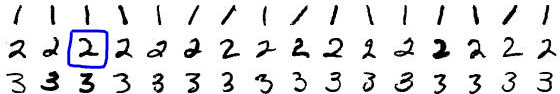
\includegraphics[width=0.7\textwidth]{figs/onetwothree}
\end{center}
\item example training procedure:
    \begin{enumerate}
    \item randomly present one image of a digit from above
\begin{center}
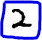
\includegraphics[width=0.1\textwidth]{figs/two} \phantom{dlasbj sadkf adsk}
\end{center}
    \item if dog barks correct number of times then gets treat

\vspace{5mm}
\hspace{10mm} \emph{bark! bark!} \qquad $\implies$

\vspace{-6mm}
\hfill 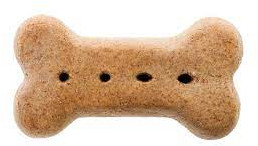
\includegraphics[width=0.15\textwidth]{figs/dogtreat} \hspace{25mm} \phantom{boo}
    \item otherwise move on to next image
    \end{enumerate}
\end{itemize}
\end{frame}


\begin{frame}{``training'' is a biologically-motivated procedure}

\begin{itemize}
\item biological learning can last from hours to decades
\item something permanent changes within the brain
    \begin{itemize}
    \item[$\circ$] neuron excitation is electrical (activation is temporary)
    \item[$\circ$] neuron count is relatively fixed
    \item[$\circ$] in learning, there are chemical or morpological changes in connections between neurons, the \alert{synapses} where an axon connects to another neuron's dendrite
    \end{itemize}
\end{itemize}

\begin{center}
\mbox{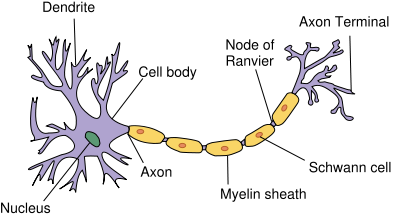
\includegraphics[width=0.5\textwidth]{figs/physicalneuron} 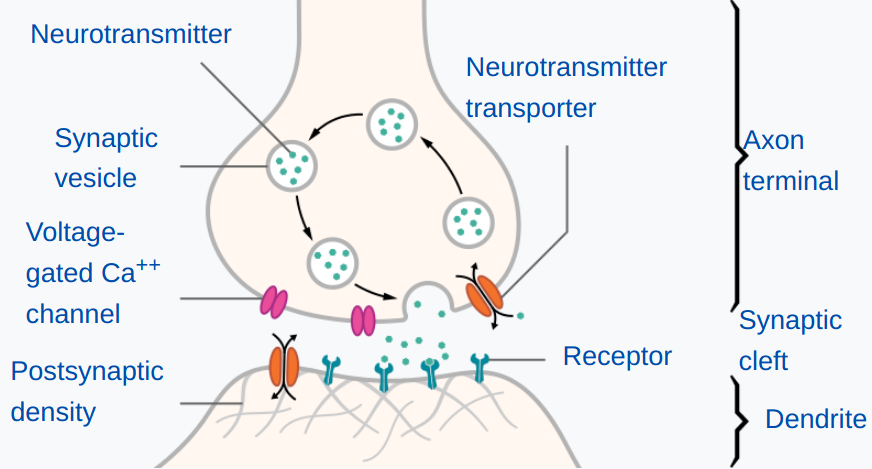
\includegraphics[width=0.4\textwidth]{figs/synapse}}
\end{center}
\end{frame}


\begin{frame}{artificial neurons as a model of real neurons}

\begin{itemize}
\item we replace all the above biological complexity with a simplified artificial neuron

\begin{center}
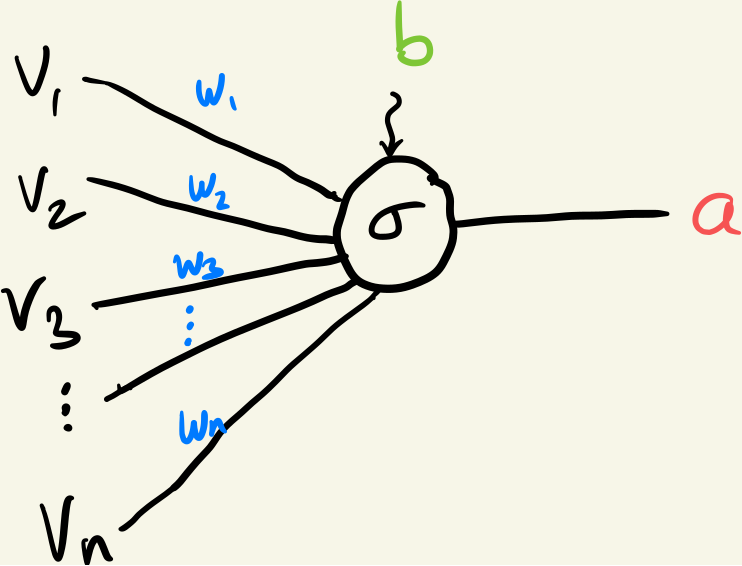
\includegraphics[width=0.3\textwidth]{figs/b-single-neuron}
\end{center}

    \begin{itemize}
    \item[$\circ$] i.e.~the model is merely a formula: \quad $\displaystyle {\color{red} a} = \sigma\left(\sum_{k=1}^{n} {\color{blue} w_{k}} x_k + {\color{ForestGreen} b}\right)$
    \end{itemize}
\item training will make ``permanent'' changes in the weights ${\color{blue} w_k}$ and biases ${\color{ForestGreen} b}$
\item after training, forward passes are ``learned behavior''
\end{itemize}
\end{frame}


\begin{frame}{training $=$ nonlinear least-squares optimization}

\begin{itemize}
\item so, how does training work in artificial neural networks?
\end{itemize}
\end{frame}


\section{backward through a neural net}

\begin{frame}{Outline}
  \tableofcontents[hideallsubsections,currentsection]
\end{frame}


\begin{frame}{fixme}

\begin{itemize}
\item latex
\item beamer
\end{itemize}
\end{frame}


\section{running the codes yourself}

\begin{frame}{Outline}
  \tableofcontents[hideallsubsections,currentsection]
\end{frame}


\begin{frame}{\emph{Matlab online} instructions: HH19 codes}

\begin{itemize}
\item as a UAF person you have access to Matlab online if you want it

\begin{center}
\href{https://matlab.mathworks.com/}{\texttt{matlab.mathworks.com}}
\end{center}

    \begin{itemize}
    \item[$\circ$] I also use Octave
    \end{itemize}
\item 
\item beamer
\end{itemize}
\end{frame}


\begin{frame}{\emph{Matlab online} instructions: my versions of HH19 codes}

\begin{itemize}
\item FIXME
\item beamer
\end{itemize}
\end{frame}


\section{things that bother me}

\begin{frame}{Outline}
  \tableofcontents[hideallsubsections,currentsection]
\end{frame}


\begin{frame}{fixme}

\begin{itemize}
\item latex
\item beamer
\end{itemize}
\end{frame}

\end{document}
